\chapter{Introducción}

Las \textbf{API} (en inglés “\textit{application programming interface}”) son hoy en día una parte fundamental de servicios y aplicaciones. Nos permite obtener datos, comunicar aplicaciones entre sí, y realizar una separación entre la parte lógica de la aplicación y la parte visual, pudiendo ser esta última una aplicación web, una de móvil, de televisión...

Es por eso que aprender y entender cómo crear una API es una parte fundamental que todo programador debe conocer, ya que de esta manera vamos a entender de mejor manera cómo funcionan. Esto nos será muy útil también, incluso, para utilizarlas.

Por todo ello, a continuación se va a explicar cómo hacer que nuestra aplicación cuente con API, para poder ser utilizada desde otra aplicación o para ser utilizada para obtener datos desde otro tipo de interfaz. Para ello, cabe recordar que las peticiones y los resultados deben ir en formato \href{https://es.wikipedia.org/wiki/JSON}{JSON}.


\chapter{Rutas para la API}

Hasta ahora hemos hecho uso del fichero \configfile{routes/web.php} para añadir rutas a nuestra aplicación. En el mismo directorio podemos ver que existe otro fichero llamado \configfile{routes/api.php}, que, como su propio nombre indica, vamos a utilizar para añadir las rutas que utilizaremos en nuestra API.

Si observamos el fichero, vemos ya existe una ruta creada:

\begin{mycode}{Contenido del fichero web.php}{php}{{\small }}
<?php
use Illuminate\Http\Request;
use Illuminate\Support\Facades\Route;

Route::middleware('auth:sanctum')->get('/user', function (Request $request) {
    return $request->user();
});
\end{mycode}

Si obtenemos el listado de rutas, veremos que ya existe una ruta para conocer el estado del usuario. A continuación vamos a añadir las rutas correspondientes para toda la gestión de los “posts” de nuestra aplicación.

Debemos recordar que para poder añadir las nuevas rutas, hay que incluir el controlador correspondiente, en este caso el \textbf{PostController}.

\begin{mycode}{Añadir nuevas rutas al fichero web.php}{php}{}
<?php
...
use App\Http\Controllers\PostController;
Route::resources([
    'posts' => PostController::class,
]);
\end{mycode}

Si ahora visualizamos el listado de rutas completo veremos las nuevas rutas. Si sólo nos interesan las rutas específicas a la API, podemos añadir un parámetro indicando sólo parte de la ruta, como se muestra a continuación:


\begin{mycode}{Añadir nuevas rutas al fichero web.php}{console}{{\small }}
root@5cff1feaf785:/var/www/html# php artisan route:list --path=api

GET|HEAD        api/posts ............ posts.index › PostController@index
POST            api/posts ............ posts.store › PostController@store
GET|HEAD        api/posts/create ..... posts.create › PostController@create
GET|HEAD        api/posts/{post} ..... posts.show › PostController@show
PUT|PATCH       api/posts/{post} ..... posts.update › PostController@update
DELETE          api/posts/{post} ..... posts.destroy › PostController@destroy
GET|HEAD        api/posts/{post}/edit  posts.edit › PostController@edit
GET|HEAD        api/user ....................................................
\end{mycode}


\chapter{Uso de controladores para la API}

Para que la modificación previa funcione es necesario modificar el controlador, ya que actualmente sólo devuelve la vista en formato código HTML. Por tanto, si queremos utilizar el mismo controlador, deberemos modificar las funciones. En el caso de la función “index” del PostController queda:


\begin{mycode}{Modificar la función de PostController}{php}{}
<?php
...
public function index(Request $request) {
    $posts = Post::orderBy('created_at')->get();
    if ($request->expectsJson()) {
        return response()->json($posts);
    } else {
        return view('posts.index',['posts' => $posts]);
    }
}
\end{mycode}

Tal como se puede ver, la función recibe dos modificaciones:

\begin{itemize}
    \item \textbf{Añadir parámetro “Request”}: De esta manera, podremos conocer si la petición viene desde la web, o si por el contrario se espera la respuesta en formato JSON.

    \item \textbf{Comprobar qué se espera}: Tal como se puede ver, se ha añadido un “if” donde se mira si la petición se espera en formato JSON (“expectsJson()”). En caso afirmativo, se devuelve la respuesta correspondiente en formato JSON.
\end{itemize}

\errorbox{\textbf{Es recomendable hacer uso de controladores específicos}}



\section{Crear controladores específicos}

Debido a que las API se suelen versionar, es recomendable mantener los controladores de la web y de la API separados. Esto permite seguir el principio \textbf{\textit{KISS}} (\textit{Keep It Simple, Stupid!}). De esta manera se va a poder realizar modificaciones en un apartado de nuestra aplicación sin temer que podemos romper otra parte.

Es por ello, que lo ideal es crear controladores específicos para las funcionalidades que va a tener la API, y que se encuentren separados. Para ello realizaremos lo siguiente:

\begin{itemize}
    \item \textbf{Deshacer los cambios} de la función “index” vistos en el apartado anterior.
    \item \textbf{Crear nuevo controlador} que será específico para la API:

\begin{mycode}{Crear nuevo PostController exclusivo para la API}{console}{{\small}}
# php artisan make:controller API/PostController --api --model=Post
\end{mycode}

    Es necesario explicar lo siguiente:
    \begin{itemize}
        \item \textbf{“API/PostController”}: Esto indica cuál es la ruta donde se creará el fichero, que en este caso es \configfile{app/Http/Controllers/API/PostController.php}.

       \item \textbf{\texttt{--api}}: Este parámetro va a generar un controlador que carece de las funciones “create” y “edit”, ya que no son necesarias en una API, dado que son exclusivas a visualizar los formularios en un interfaz web.

       \item \textbf{\texttt{--model=Post}}: Para que el nuevo fichero del controlador ya tenga el include del modelo necesario.
    \end{itemize}

    \item \textbf{Modificar la ruta para la API} y que de esta manera haga uso del nuevo controlador exclusivo. El cambio

\begin{mycode}{Modificar api.php para el nuevo controlador}{php}{}
<?php
...
use App\Http\Controllers\API\PostController;
\end{mycode}

    \item Modificar nuevo controlador, para que devuelva los datos correspondientes:

\begin{mycode}{Modificar api.php para el nuevo controlador}{php}{}
<?php
...
public function index(){
    $posts = Post::orderBy('created_at')->get();
    return response()->json($posts);
}
\end{mycode}

\end{itemize}


\chapter{Comprobar funcionamiento}
Es momento de comprobar que todo funciona de manera correcta, y para ello debemos realizar una petición a la URL \href{http://localhost/api/posts}{http://localhost/api/posts} teniendo en cuenta el ejemplo que hemos estado realizando.

Para realizar la prueba podemos hacerlo de distintas formas, cada una de ellas dependiendo de la motivación que tengamos:

\begin{itemize}
    \item Desde el propio \textbf{navegador web}. Veremos los datos JSON devueltos en formato texto directamente. Para comprobar que funciona, puede ser más que suficiente.

    \item Desde una \textbf{consola Linux}, haciendo uso del comando \textbf{curl}, podemos también comprobar de manera rápida si el \textit{endpoint} está funcionando:

\begin{mycode}{Modificar api.php para el nuevo controlador}{console}{}
ruben@vega:~$ curl -s  http://localhost/api/posts
[{"id":1,"titulo":"Primer post","texto":"Este..."...}]
\end{mycode}

    Si queremos tener un resultado más visual, podremos hacer uso del comando “\textbf{jq}”, que deberemos instalarlo. De esta manera, podremos hacer:

\begin{mycode}{Modificar api.php para el nuevo controlador}{console}{}
ruben@vega:~$ curl -s  http://localhost/api/posts | jq
[
  {
    "id": 1,
    "titulo": "Primer post",
    "texto": "Este es el texto del primer post",
    "publicado": 1,
    "deleted_at": null,
    "created_at": "2023-10-04T08:20:29.000000Z",
    "updated_at": "2023-11-16T08:08:27.000000Z"
  }
]
\end{mycode}

    \item Utilizando un interfaz gráfico como \href{https://www.postman.com/}{Postman}, que nos va a facilitar hacer peticiones GET y peticiones más complejas.

    \begin{center}
        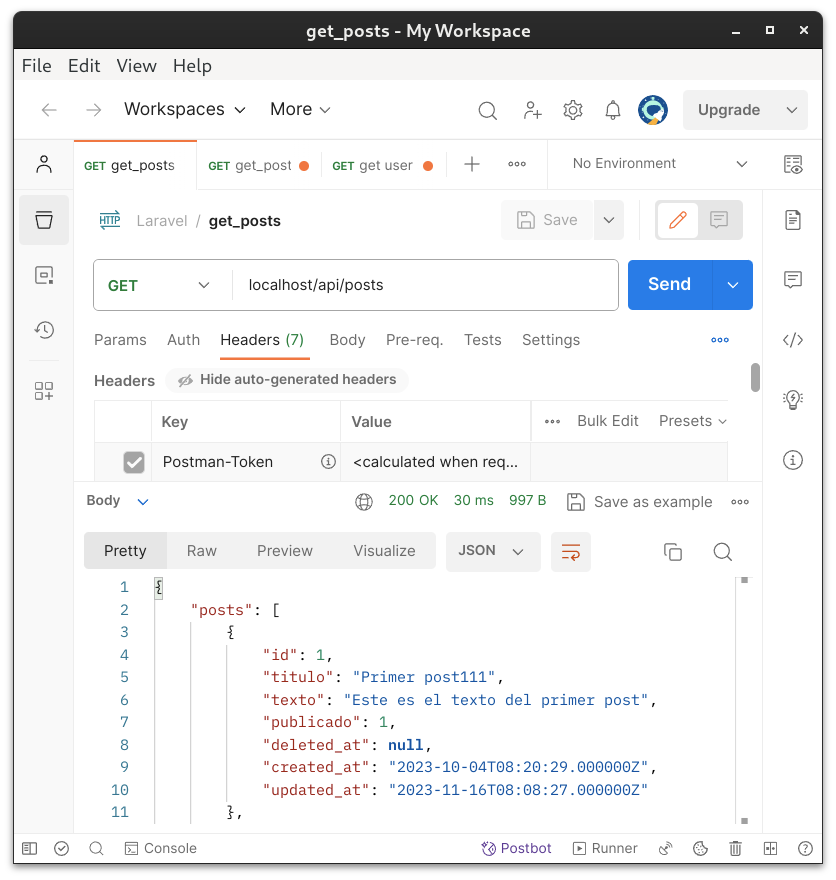
\includegraphics[width=0.8\linewidth]{postman.png}
    \end{center}

\end{itemize}


\chapter{Visualizar API}

Suele ser habitual tener un interfaz donde se muestra el funcionamiento de nuestra API, o cuáles son los \textit{endpoints} de la misma. Es decir, qué URL se pueden consultar, qué método hay que utilizar, si es necesario el paso de parámetros, ...

Hoy en día existe la especificación \href{https://www.openapis.org/}{OpenAPI} para la generación de la API, y sobre ella existen distintos interfaces web. Uno de los interfaces más utilizados es \href{https://swagger.io/tools/swagger-ui/}{Swagger UI} que nos muestra un bonito interfaz y a la vez es posible utilizarlo para realizar consultas a la API.

Para poder instalarlo en nuestro proyecto Laravel, necesitamos realizar la instalación de unas dependencias y la posterior instalación en el proyecto.

\begin{mycode}{Instalación de dependencias}{console}{{\small}}
root@5cff1feaf785:/var/www/html# composer require "darkaonline/l5-swagger"

root@5cff1feaf785:/var/www/html# php artisan vendor:publish \
    --provider "L5Swagger\L5SwaggerServiceProvider"
\end{mycode}


Ahora deberemos añadir comentarios a las funciones para poder generar el interfaz de manera correcta. En uno de los controladores añadiremos la siguiente cabecera (\textbf{sólo es necesario añadirlo en un controlador}):

\begin{mycode}{Cabecera para la API}{php}{}
<?php
/**
* @OA\Info(title="API", version="1.0")
*/
\end{mycode}


Para documentar la función \textbf{index}, encima de ella añadiremos lo siguiente:

\begin{mycode}{Comentario para /api/posts}{php}{}
<?php
...
/**
* @OA\Get(
*     path="/api/posts",
*     summary="Mostrar posts",
*     @OA\Response(
*         response=200,
*         description="Mostrar todos los posts."
*     ),
*     @OA\Response(
*         response="default",
*         description="Ha ocurrido un error."
*     )
* )
*/
public function index(){
//...
\end{mycode}

Y para la función \textbf{show}, que sólo nos muestra un único post, añadiremos los siguientes comentarios:

\begin{mycode}{Comentario para /api/posts/ID}{php}{}
<?php
...
/**
* @OA\Get(
*     path="/api/posts/{id}",
*     summary="Mostrar un post concreto",
*     @OA\Parameter(
*          name="id",
*          description="Project id",
*          required=true,
*          in="path",
*          @OA\Schema(
*              type="integer"
*          )
*     ),
*     @OA\Response(
*         response=200,
*         description="Mostrar el post especificado."
*     ),
*     @OA\Response(
*         response="default",
*         description="Ha ocurrido un error."
*     )
* )
*/
public function show(Post $post) {
//...
\end{mycode}

Tras esto, ejecutaremos el comando que recorrerá los controladores para generar el fichero \configfile{storage/api-docs/api-docs.json}:

\begin{mycode}{Generamos el fichero json para Swagger}{console}{}
root@5cff1feaf785:/var/www/html# php artisan l5-swagger:generate
Regenerating docs default
\end{mycode}

Para conocer todas las funcionalidades de los comentarios, es recomendable mirar la \href{https://github.com/zircote/swagger-php#usage}{documentación}. Tras ejecutar el comando anterior, si vamos a la url \href{http://localhost/api/documentation}{http://localhost/api/documentation} tendremos acceso y veremos el interfaz para nuestra API:

\begin{center}
    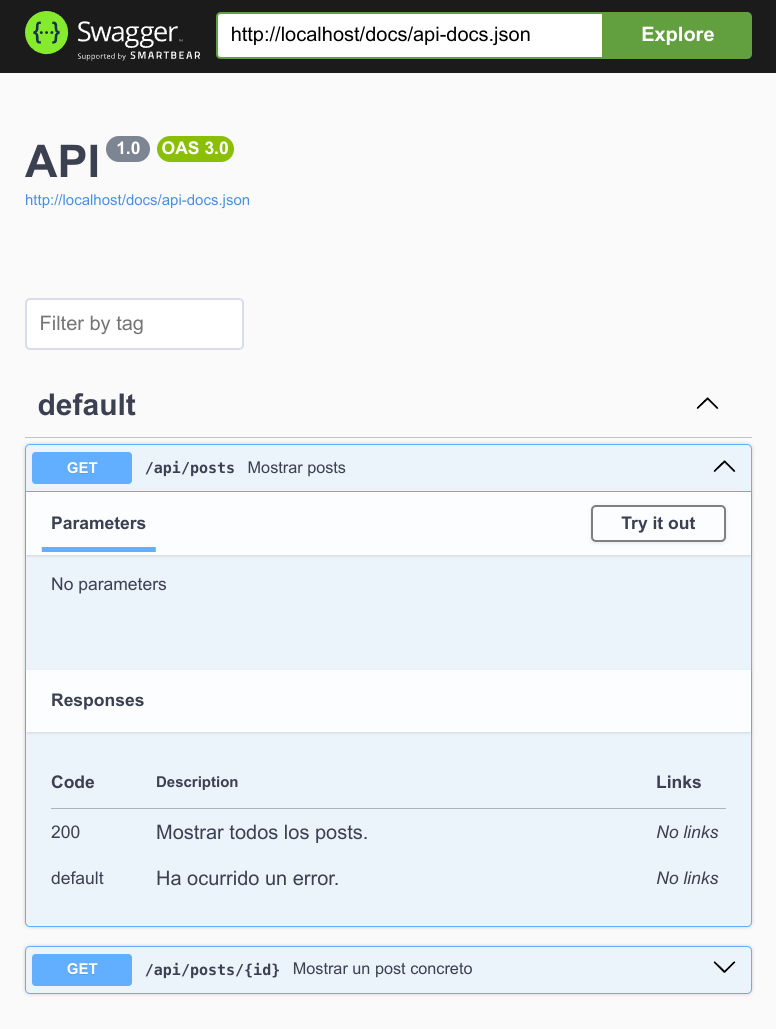
\includegraphics[frame,width=0.7\linewidth]{swagger.png}
\end{center}

% Mostrar SWAGGER.io
% https://styde.net/como-documentar-una-api-en-laravel-usando-swagger/
% https://github.com/DarkaOnLine/L5-Swagger
% https://github.com/zircote/swagger-php
% https://zircote.github.io/swagger-php/




% Certificados y JWT


%\chapter{Versionar API}
% https://laravel.io/articles/api-versioning-in-laravel
% https://dev.to/dalelantowork/laravel-8-api-versioning-4e8